% !TeX program = xelatex
\ifdefined\BookMaster\else
\documentclass[11pt,oneside]{article}
% !TeX program = xelatex
\usepackage[b5paper,left=22mm,right=22mm,top=20mm,bottom=22mm,footskip=11mm]{geometry}
\usepackage{fontspec}
\setmainfont{TeX Gyre Termes}
\setsansfont{TeX Gyre Heros}
\usepackage{amsmath,amssymb,mathtools,amsthm}
\renewcommand{\cdots}{\mathinner{\cdotp\cdotp\cdotp}}
\usepackage{graphicx,adjustbox,array,booktabs,longtable,multirow,enumitem,changepage,needspace}
\usepackage[table]{xcolor}
\usepackage{fancyhdr}
\raggedbottom
\interfootnotelinepenalty=10000
\newcommand{\BookFootnote}[2]{\begingroup\renewcommand{\thefootnote}{\fnsymbol{footnote}}\footnote[#1]{#2}\endgroup}
\newcommand{\BookFootnoteMark}[1]{\begingroup\renewcommand{\thefootnote}{\fnsymbol{footnote}}\footnotemark[#1]\endgroup}
\newcommand{\BookFootnoteText}[2]{\begingroup\renewcommand{\thefootnote}{\fnsymbol{footnote}}\footnotetext[#1]{#2}\endgroup}
\newenvironment{BookFloat}[1]{\par\addvspace{.6\baselineskip}\noindent\def\BookFloatID{#1}\begin{minipage}{\linewidth}\phantomsection\label{bookfloat:#1:start}}{\phantomsection\label{bookfloat:\BookFloatID:end}\end{minipage}\par\addvspace{.6\baselineskip}}

\usepackage[unicode,hidelinks]{hyperref}
\pagestyle{fancy}
\fancyhf{}
\newcommand{\BookFooter}{}
\fancyfoot[L]{\parbox[b]{\dimexpr\textwidth-15mm}{\footnotesize\BookFooter}}
\fancyfoot[R]{\footnotesize\thepage}
\renewcommand{\headrulewidth}{0pt}
\renewcommand{\footrulewidth}{0pt}
\setlength{\parindent}{0pt}
\setlength{\parskip}{0.2em}
\setlength{\emergencystretch}{3em}
\setlist{nosep,leftmargin=1.7em,labelsep=.65em}
\newif\ifBookNarrative
\BookNarrativetrue
\newenvironment{BookBody}{\setlength{\parindent}{0pt}}{}
\newcommand{\BookStatement}[1]{\par\addvspace{.6\baselineskip}\noindent #1\enspace\ignorespaces}
\newcommand{\BookLabel}[1]{\par\addvspace{.6\baselineskip}\needspace{3\baselineskip}\noindent\textbf{#1}\quad\ignorespaces}
\newcommand{\BookHeading}[1]{\par\addvspace{\baselineskip}\needspace{4\baselineskip}\noindent{\large\bfseries #1}\par\medskip}
\newcommand{\BookSubheading}[1]{\par\addvspace{.7\baselineskip}\needspace{3\baselineskip}\noindent{\bfseries #1}\par\smallskip}
\newcommand{\BookTextHeading}[1]{\par\addvspace{.7\baselineskip}\needspace{3\baselineskip}\noindent #1\par\smallskip}
\newcommand{\BookSectionTitle}[2]{\par\addvspace{1.2\baselineskip}\needspace{5\baselineskip}\noindent\colorbox{gray!25}{\sffamily\bfseries\small SECTION #1}\quad{\large\bfseries #2}\par\medskip}
\newcommand{\BookExerciseTitle}[1]{\par\addvspace{\baselineskip}\needspace{4\baselineskip}\noindent{\color{gray}\rule{1.5mm}{1.5mm}}\enspace{\large\bfseries Exercises #1}\par\medskip}
\newcommand{\BookBullet}[1]{\begin{list}{\textbullet}{\setlength{\leftmargin}{1.7em}\setlength{\labelwidth}{1em}\setlength{\labelsep}{.7em}\setlength{\topsep}{0pt}\setlength{\parsep}{0pt}\setlength{\itemsep}{0pt}}\item #1\end{list}}
\newcommand{\BookExercise}[2]{\begin{list}{\textbf{#1}}{\setlength{\leftmargin}{2.2em}\setlength{\labelwidth}{1.5em}\setlength{\labelsep}{.7em}\setlength{\topsep}{.15em}\setlength{\parsep}{0pt}\setlength{\itemsep}{0pt}}\item #2\end{list}}
\newcommand{\BookEnd}[1]{\unskip\nobreak\hfill\ensuremath{#1}}
\newcommand{\BookSource}[2]{\phantomsection\label{sourcepage:#1}} % Source-page anchors, retained through reflow.
\usepackage{multicol}
\usepackage{tikz}
\newcommand{\BookPartEntry}[2]{\par\noindent\makebox[17mm][l]{\bfseries Section #1}#2\par}
\newcommand{\BookPartTitle}[3]{\par\bigskip\noindent\begin{tikzpicture}\node[anchor=north west,inner sep=0pt,outer sep=0pt] (bookpart) at (0,0) {\begin{minipage}{\dimexpr\linewidth-.5pt}\hspace*{26mm}\begin{minipage}[t]{\dimexpr\linewidth-26mm}\begin{adjustbox}{max width=\linewidth}{\fontsize{20}{24}\selectfont\bfseries #2}\end{adjustbox}\par\vspace{6mm}\hrule\vspace{6mm}{\sffamily\footnotesize\setlength{\parskip}{.3em}#3}\vspace{3mm}\end{minipage}\end{minipage}};\path[shade,top color=gray!60,bottom color=white] (0,0) rectangle ([xshift=24mm]bookpart.south west);\node[anchor=north,font=\sffamily\bfseries\small] at (12mm,-2mm) {PART};\node[anchor=north,font=\sffamily\bfseries\Huge] at (12mm,-7mm) {#1};\end{tikzpicture}\par\bigskip}
\newsavebox{\BookMathBox}
\makeatletter
\newcommand{\BookInline}[1]{\leavevmode\hskip0pt\relax\begingroup\in@{\begin}{#1}\ifin@\sbox{\BookMathBox}{\(#1\)}\ifdim\wd\BookMathBox>\dimexpr\linewidth-1em\relax\resizebox{\dimexpr\linewidth-1em\relax}{!}{\usebox{\BookMathBox}}\else\(#1\)\fi\else\in@{\left}{#1}\ifin@\sbox{\BookMathBox}{\(#1\)}\ifdim\wd\BookMathBox>\dimexpr\linewidth-1em\relax\resizebox{\dimexpr\linewidth-1em\relax}{!}{\usebox{\BookMathBox}}\else\(#1\)\fi\else\(#1\)\fi\fi\endgroup\hskip0pt\relax}
\makeatother
\DeclareMathOperator{\Aut}{Aut}
\DeclareMathOperator{\End}{End}
\DeclareMathOperator{\Hom}{Hom}
\DeclareMathOperator{\GF}{GF}
\DeclareMathOperator{\irr}{irr}
\DeclareMathOperator{\lt}{lt}
\DeclareMathOperator{\lp}{lp}
\providecommand{\textcircled}[1]{\textnormal{(#1)}}

\begin{document}
\fi
\renewcommand{\BookFooter}{Section 41 Geometric Constructions}
\pdfbookmark[0]{Section 41 Geometric Constructions}{41_geometric_constructions}
\ifdefined\BookMaster\else\setcounter{page}{328}\fi
% Source PDF page 345; original printed page 328
\BookSource{345}{328}
\BookNarrativetrue

\begin{BookBody}

\BookSectionTitle{41}{Geometric Constructions\label{bookfootnote:345:2:ref}\BookFootnote{2}{\label{bookfootnote:345:2:text}This section is used only briefly in Section 48.}}

\noindent In this section we digress briefly to give an application demonstrating the power of Theorem 40.4. For a more detailed study of geometric constructions, you are referred to Courant and Robbins [44, Chapter III].

In Euclid’s\textit{ Elements}, geometry is approached from an axiomatic point of view. The first three axioms state that a line segment can be drawn between any two given points, 
% Source PDF page 346; original printed page 329
\BookSource{346}{329}
a line segment can be extended indefinitely to form a line, and a circle can be drawn centered at any given point with any given radius. A straightedge and a compass are objects that can accomplish the tasks set out in these axioms. A natural question asked by the ancient Greek geometers was exactly which points and configurations can be constructed using only a compass and a straightedge. They found many constructions that are well known today including bisecting angles, bisecting line segments, and trisecting line segments. Trisecting an arbitrary angle eluded mathematicians for well over 2000 years before field theory was developed and it was proven that there are some angles that are impossible to trisect using only a straightedge and compass. We shall discuss the impossibility of trisecting an angle and other classical questions.

\end{BookBody}

\BookNarrativetrue

\begin{BookBody}

\BookTextHeading{\textbf{Constructible Numbers}  }

\noindent Let us imagine that we are given only a single line segment that we shall define to be \textit{one unit} in length. A real number \BookInline{\alpha } is\textbf{ constructible} if we can construct a line segment of length \BookInline{|\alpha |} in a finite number of steps from this given segment of unit length by using a straightedge and a compass.

The rules of the game are pretty strict. We suppose that we are given just two points at the moment, the endpoints of our unit line segment, let us suppose that they correspond to the points (0, 0) and (1, 0) in the Euclidean plane. We are allowed to draw a line only with our straightedge through two points that we have already located. Thus we can start by using the straightedge and drawing the line through (0, 0) and (1, 0). We are allowed to open our compass only to a distance between points we have already found. Let us open our compass to the distance between (0, 0) and (1, 0). We can then place the point of the compass at (1, 0) and draw a circle of radius 1, which passes through the point (2, 0). Thus we now have located a third point, (2, 0). Continuing in this way, we can locate points \BookInline{(3,\allowbreak 0),\allowbreak (4,\allowbreak 0),\allowbreak (- 1,\allowbreak 0),\allowbreak (- 2,\allowbreak 0),\allowbreak } and so on. Now open the compass the distance from (0, 0) to (0, 2), put the point at (1, 0), and draw a circle of radius 2. Do the same with the point at \BookInline{(- 1,\allowbreak 0).} We have now found two new points, where these circles intersect, and we can put our straightedge on them to draw what we think of as the \BookInline{y-}axis. Then opening our compass to the distance from (0, 0) to (1, 0), we draw a circle with center at (0, 0) and locate the point (0, 1) where the circle intersects the \BookInline{y-}axis. Continuing in this fashion, we can locate all points \BookInline{(x,\allowbreak y)} with integer coordinates in any rectangle containing the point (0, 0). Without going into more detail, it can be shown that it is possible, among other things, to erect a perpendicular to a given line at a known point on the line, and find a line passing through a known point and parallel to a given line. Our first result is the following theorem.

\BookLabel{41.1 Theorem} If \BookInline{\alpha } and \BookInline{\beta } are constructible real numbers, then so are \BookInline{\alpha + \beta,\allowbreak \alpha - \beta,\allowbreak \alpha \beta,\allowbreak } and \BookInline{\alpha /\beta,\allowbreak } if \BookInline{\beta \neq 0.}

\BookLabel{\textit{Proof}} We are given that \BookInline{\alpha } and \BookInline{\beta } are constructible, so there are line segments of lengths \BookInline{|\alpha |} and \BookInline{|\beta |} available to us. For \BookInline{\alpha,\allowbreak \beta >0,\allowbreak } extend a line segment of length \BookInline{\alpha } with the straightedge. Start at one end of the original segment of length \BookInline{\alpha,\allowbreak } and lay off on the extension the length \BookInline{\beta } with the compass. This constructs a line segment of length \BookInline{\alpha + \beta;\alpha - \beta } is similiarly constructible (see Fig. 41.2). If \BookInline{\alpha } and \BookInline{\beta } are not both positive, an obvious

\begin{BookFloat}{41_geometric_constructions-p346-6}
\begin{center}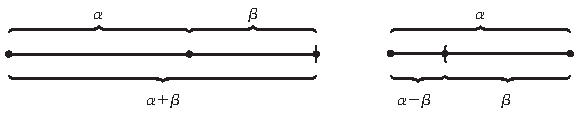
\includegraphics[width=0.793\linewidth,height=.8\textheight,keepaspectratio]{assets/p346_07.pdf}\end{center}
\begin{center}\small\textbf{41.2 Figure}\end{center}
\end{BookFloat}

\end{BookBody}

% Source PDF page 347; original printed page 330
\BookSource{347}{330}
\BookNarrativetrue

\begin{BookBody}

\noindent breakdown into cases according to their signs shows that \BookInline{\alpha + \beta } and \BookInline{\alpha - \beta } are still constructible.

The construction of \BookInline{\alpha \beta } is indicated in Fig. 41.3. We shall let \BookInline{O\overline{A}} be the line segment from the point \BookInline{O} to the point \BookInline{A,\allowbreak } and shall let \BookInline{|OA|} be the length of this line segment. If \BookInline{O\overline{A}} is of length \BookInline{|\alpha |,\allowbreak } construct a line \BookInline{l} through \BookInline{O} not containing \BookInline{O\overline{A}.(}Perhaps, if \BookInline{O} is at (0, 0) and \BookInline{A} is at \BookInline{(a,\allowbreak 0),\allowbreak } you use the line through (0, 0) and (4, 2).) Then find the points \BookInline{P} and \BookInline{B} on \BookInline{l} such that\textit{ OP} is of length 1 and\textit{ OB} is of length \BookInline{|\beta |.} Draw\textit{ PA} and construct \BookInline{l^{\prime }} through \BookInline{B,\allowbreak } parallel to\textit{ PA} and intersecting \BookInline{OA} extended at \BookInline{Q.} By similar triangles, we have

\begin{center}\begin{adjustbox}{max width=\linewidth}\BookInline{\displaystyle { \frac { 1 } { | \alpha | } } = { \frac { | \beta | } { | { \overline { { O Q } } } | } } ,\allowbreak }\end{adjustbox}\end{center}

\noindent so \BookInline{O\overline{Q}} is of length \BookInline{|\alpha \beta |.}

\begin{BookFloat}{41_geometric_constructions-p347-4}
\begin{center}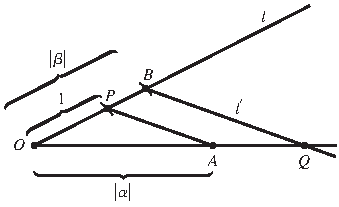
\includegraphics[width=0.466\linewidth,height=.8\textheight,keepaspectratio]{assets/p347_04.pdf}\end{center}
\begin{center}\small\textbf{41.3 Figure}\end{center}
\end{BookFloat}

Finally, Fig. 41.4 shows that \BookInline{\alpha /\beta } is constructible if \BookInline{\beta \neq 0.} Let \BookInline{O\overline{A}} be of length \BookInline{|\alpha |,\allowbreak } and construct \BookInline{l} through \BookInline{O} not containing \BookInline{OA.} Then find \BookInline{B} and \BookInline{P} on \BookInline{l} such that\textit{ OB} is of length \BookInline{|\beta |} and\textit{ OP} is of length 1. Draw \BookInline{BA} and construct \BookInline{l^{\prime }} through \BookInline{P,\allowbreak } parallel to \BookInline{BA,\allowbreak } and intersecting \BookInline{OA} at \BookInline{Q.} Again by similar triangles, we have

\begin{center}\begin{adjustbox}{max width=\linewidth}\BookInline{\displaystyle { \frac { | { \overline { { O Q } } } | } { 1 } } = { \frac { | \alpha | } { | \beta | } } ,\allowbreak }\end{adjustbox}\end{center}

\noindent so \BookInline{O\overline{Q}} is of length \BookInline{|\alpha /\beta |.} \BookEnd{\blacklozenge}

\begin{BookFloat}{41_geometric_constructions-p347-9}
\begin{center}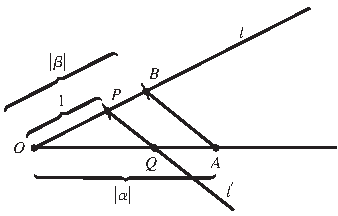
\includegraphics[width=0.464\linewidth,height=.8\textheight,keepaspectratio]{assets/p347_09.pdf}\end{center}
\begin{center}\small\textbf{41.4 Figure}\end{center}
\end{BookFloat}

\BookLabel{41.5 Corollary} The set of all constructible real numbers forms a subfield \BookInline{F} of the field of real numbers.

\BookLabel{\textit{Proof}} Proof of this corollary is immediate from Theorem 41.1. \BookEnd{\blacklozenge}

Thus the field \BookInline{F} of all constructible real numbers contains \BookInline{\mathbb{Q},\allowbreak } the field of rational numbers, since \BookInline{\mathbb{Q}} is the smallest subfield of \BookInline{\mathbb{R}.}

\end{BookBody}

% Source PDF page 348; original printed page 331
\BookSource{348}{331}
\BookNarrativetrue

\begin{BookBody}

From now on, we proceed analytically. We can construct any rational number. Regarding our given segment

0 1

\noindent of length 1 as the basic unit on an \BookInline{x-}axis, we can locate any point \BookInline{(q_{1},\allowbreak q_{2})} in the plane with both coordinates rational. Any further point in the plane that we can locate by using a compass and a straightedge can be found in one of the following three ways:

\BookExercise{1.}{as an intersection of two lines, each of which passes through two known points having rational coordinates,}

\BookExercise{2.}{as an intersection of a line that passes through two points having rational coordinates and a circle whose center has rational coordinates and whose radius is rational.}

\BookExercise{3.}{as an intersection of two circles whose centers have rational coordinates and whose radii are rational.}

Equations of lines and circles of the type discussed in 1, 2, and 3 are of the form

\begin{center}\begin{adjustbox}{max width=\linewidth}\BookInline{\displaystyle ax+ by+ c= 0}\end{adjustbox}\end{center}

\noindent and

\begin{center}\begin{adjustbox}{max width=\linewidth}\BookInline{\displaystyle x^{2}+ y^{2}+ dx+ ey+ f= 0,\allowbreak }\end{adjustbox}\end{center}

\noindent where \BookInline{a,\allowbreak b,\allowbreak c,\allowbreak d,\allowbreak e,\allowbreak } and \BookInline{f} are all in \BookInline{\mathbb{Q}.} Since in Case 3 the intersection of two circles with equations

\begin{center}\begin{adjustbox}{max width=\linewidth}\BookInline{\displaystyle x^{2}+ y^{2}+ d_{1}x+ e_{1}y+ f_{1}= 0}\end{adjustbox}\end{center}

\noindent and

\begin{center}\begin{adjustbox}{max width=\linewidth}\BookInline{\displaystyle x^{2}+ y^{2}+ d_{2}x+ e_{2}y+ f_{2}= 0}\end{adjustbox}\end{center}

\noindent is the same as the intersection of the first circle having equation

\begin{center}\begin{adjustbox}{max width=\linewidth}\BookInline{\displaystyle x^{2}+ y^{2}+ d_{1}x+ e_{1}y+ f_{1}= 0,\allowbreak }\end{adjustbox}\end{center}

\noindent and the line (the common chord) having equation

\begin{center}\begin{adjustbox}{max width=\linewidth}\BookInline{\displaystyle (d_{1}- d_{2})x+ (e_{1}- e_{2})y+ f_{1}- f_{2}= 0,\allowbreak }\end{adjustbox}\end{center}

\noindent we see that Case 3 can be reduced to Case 2. For Case 1, a simultaneous solution of two linear equations with rational coefficients can only lead to rational values of \BookInline{x} and \BookInline{y,\allowbreak } giving us no new points. However, finding a simultaneous solution of a linear equation with rational coefficients and a quadratic equation with rational coefficients, as in Case 2, leads, upon substitution, to a quadratic equation. Such an equation, when solved by the quadratic formula, may have solutions involving square roots of numbers that are not squares in \BookInline{\mathbb{Q}.}

In the preceding argument, nothing was really used involving \BookInline{\mathbb{Q}} except field axioms. If \BookInline{H} is the smallest field containing those real numbers constructed so far, the argument shows that the “next new number” constructed lies in a field \BookInline{H(\sqrt{\alpha })} for some \BookInline{\alpha \in H,\allowbreak } where \BookInline{\alpha >0.} We have proved half of our next theorem.

\BookLabel{41.6 Theorem} The field \BookInline{F} of constructible real numbers consists precisely of all real numbers that we can obtain from \BookInline{\mathbb{Q}} by taking square roots of positive numbers a finite number of times and applying a finite number of field operations.

\BookLabel{\textit{Proof}} We have shown that \BookInline{F} can contain no numbers except those we obtain from \BookInline{\mathbb{Q}} by taking a finite number of square roots of positive numbers and applying a finite number 
% Source PDF page 349; original printed page 332
\BookSource{349}{332}
of field operations. However, if \BookInline{\alpha >0} is constructible, then Fig. 41.7 shows that \BookInline{\sqrt{\alpha }} is constructible. Let \BookInline{O\overline{A}} have length \BookInline{\alpha,\allowbreak } and find \BookInline{P} on \BookInline{O\overline{A}} extended so that\textit{ OP} has length 1. Find the midpoint of\textit{ PA} and draw a semicircle with\textit{ PA} as diameter. Erect a perpendicular to\textit{ PA} at \BookInline{O,\allowbreak } intersecting the semicircle at \BookInline{Q.} Then the triangles \BookInline{OPQ} and \BookInline{OQA} are similar, so

\end{BookBody}

\BookNarrativetrue

\begin{BookBody}

\begin{center}\begin{adjustbox}{max width=\linewidth}\BookInline{\displaystyle \frac { | \overline { { O Q } } | } { | \overline { { O A } } | } = \frac { | \overline { { O P } } | } { | \overline { { O Q } } | } ,\allowbreak }\end{adjustbox}\end{center}

and \BookInline{|O\overline{Q}|^{2}= 1\alpha = \alpha.} Thus \BookInline{O\overline{Q}} is of length \BookInline{\sqrt{\alpha }.} Therefore square roots of constructible numbers are constructible.

Theorem 41.1 showed that field operations are possible by construction\BookInline{.}\BookEnd{\blacklozenge}

\begin{BookFloat}{41_geometric_constructions-p349-4}
\begin{center}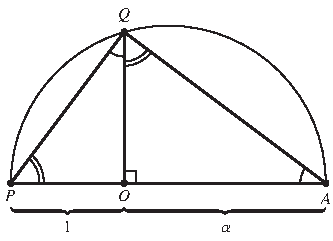
\includegraphics[width=0.457\linewidth,height=.8\textheight,keepaspectratio]{assets/p349_05.pdf}\end{center}
\begin{center}\small\textbf{41.7 Figure}\end{center}
\end{BookFloat}

\BookLabel{41.8 Corollary} If \BookInline{\gamma } is constructible and \BookInline{\gamma \notin \mathbb{Q},\allowbreak } then there is a finite sequence of real numbers \BookInline{\alpha _{1},\allowbreak \cdots,\allowbreak \alpha _{n}= \gamma } such that \BookInline{\mathbb{Q}(\alpha _{1},\allowbreak \cdots,\allowbreak \alpha _{i})} is an extension of \BookInline{\mathbb{Q}(\alpha _{1},\allowbreak \cdots,\allowbreak \alpha _{i- 1})} of degree 2. In particular\BookInline{,\allowbreak [\mathbb{Q}(\gamma ):\mathbb{Q}]= 2^{r}} for some integer \BookInline{r\geq 0.}

\BookLabel{\textit{Proof}} The existence of the \BookInline{\alpha _{i}} is immediate from Theorem 41.6. Then

\begin{center}\begin{adjustbox}{max width=\linewidth}\BookInline{\displaystyle \begin{aligned}2^{n}&= [\mathbb{Q}(\alpha _{1},\allowbreak \cdots ,\allowbreak \alpha _{n}):\mathbb{Q}] \\ &= [\mathbb{Q}(\alpha _{1},\allowbreak \cdots ,\allowbreak \alpha _{n}):\mathbb{Q}(\gamma )][\mathbb{Q}(\gamma ):\mathbb{Q}],\allowbreak \end{aligned}}\end{adjustbox}\end{center}

\noindent by Theorem 40.4, which completes the proof. \BookEnd{\blacklozenge}

\BookTextHeading{\textbf{The Impossibility of Certain Constructions}  }

\noindent We can now show the impossibility of certain geometric constructions.

\BookLabel{41.9 Theorem} \textit{Doubling the cube is impossible,} that is, given a side of a cube, it is not always possible to construct with a straightedge and a compass the side of a cube that has double the volume of the original cube.

\BookLabel{\textit{Proof}} Let the given cube have a side of length 1, and hence a volume of 1. The cube being sought would have to have a volume of 2, and hence a side of length \BookInline{\sqrt { 2 }.} But \BookInline{\sqrt { 2 }} is a zero of irreducible \BookInline{x^{3}- 2} over \BookInline{\mathbb{Q},\allowbreak } so

\begin{center}\begin{adjustbox}{max width=\linewidth}\BookInline{\displaystyle [ \mathbb { Q } ( { \sqrt [ 3 ] { 2 } } ) : \mathbb { Q } ] = 3 .}\end{adjustbox}\end{center}

\noindent Corollary 41.8 shows that to double this cube of volume 1, we would need to have \BookInline{3= 2^{r}} for some integer \BookInline{r,\allowbreak } but no such \BookInline{r} exists\BookInline{.}\BookEnd{\blacklozenge}

\end{BookBody}

% Source PDF page 350; original printed page 333
\BookSource{350}{333}
\BookNarrativetrue

\begin{BookBody}

\BookLabel{41.10 Theorem} \textit{Squaring the circle is impossible;} that is, given a circle, it is not always possible to construct with a straightedge and a compass a square having area equal to the area of the given circle.

\BookLabel{\textit{Proof}} Let the given circle have a radius of 1, and hence an area of \BookInline{\pi.} We would need to construct a square of side \BookInline{\sqrt{\pi }.} But \BookInline{\pi } is transcendental over \BookInline{\mathbb{Q},\allowbreak } so \BookInline{\sqrt{\pi }} is transcendental over \BookInline{\mathbb{Q}} also\BookInline{.}\BookEnd{\blacklozenge}

\BookLabel{41.11 Theorem} \textit{Trisecting the angle is impossible;} that is, there exists an angle that cannot be trisected with a straightedge and a compass.

\BookLabel{\textit{Proof}} Figure 41.12 indicates that the angle \BookInline{\theta } can be constructed if and only if a segment of length \BookInline{|} cos \BookInline{\theta |} can be constructed. Now \BookInline{60^{\circ }} is a constructible angle, and we shall show that it cannot be trisected. Note that

\begin{center}\begin{adjustbox}{max width=\linewidth}\BookInline{\displaystyle \begin{aligned}\;\text{cos}\;3\theta &= \;\text{cos}\;(2\theta + \theta ) \\ &= \;\text{cos}\;2\theta \;\text{cos}\;\theta - \;\text{sin}\;2\theta \;\text{sin}\;\theta  \\ &= (2\;\text{co}\;\mathrm{s}^{2}\theta - 1)\;\text{cos}\;\theta - 2\;\text{sin}\;\theta \;\text{cos}\;\theta \;\text{sin}\;\theta  \\ &= (2\;\text{co}\;\mathrm{s}^{2}\theta - 1)\;\text{cos}\;\theta - 2\;\text{cos}\;\theta (1- \;\text{co}\;\mathrm{s}^{2}\theta ) \\ &= 4\;\text{co}\;\mathrm{s}^{3}\theta - 3\;\text{cos}\;\theta .\end{aligned}}\end{adjustbox}\end{center}

\begin{BookFloat}{41_geometric_constructions-p350-5}
\begin{center}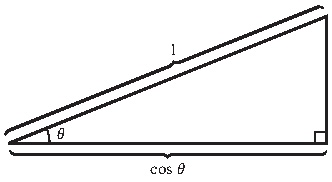
\includegraphics[width=0.455\linewidth,height=.8\textheight,keepaspectratio]{assets/p350_05.pdf}\end{center}
\begin{center}\small\textbf{41.12 Figure}\end{center}
\end{BookFloat}

[We realize that some students have not seen the trigonometric identities we just used. Exercise 1 repeats Exercise 42 of Section 3 and asks you to prove the identity cos \BookInline{3\theta = 4} cos\BookInline{3\theta - 3} cos \BookInline{\theta } from Euler’s formula.]

Let \BookInline{\theta = 20^{\circ },\allowbreak } so that cos \BookInline{3\theta = \frac{1}{2},\allowbreak } and let \BookInline{\alpha = } cos \BookInline{20^{\circ }.} From the identity 4 cos\BookInline{3\theta - } 3 cos \BookInline{\theta = } cos \BookInline{3\theta,\allowbreak } we see that

\begin{center}\begin{adjustbox}{max width=\linewidth}\BookInline{\displaystyle 4\alpha^{3}-3\alpha=\frac{1}{2}.}\end{adjustbox}\end{center}

\noindent Thus \BookInline{\alpha } is a zero of \BookInline{8x^{3}- 6x- 1.} This polynomial is irreducible in \BookInline{\mathbb{Q}[x],\allowbreak } since, by Theorem 28.12, it is enough to show that it does not factor in \BookInline{\mathbb{Z}[x].} But a factorization in \BookInline{\mathbb{Z}[x]} would entail a linear factor of the form \BookInline{(8x\pm 1),\allowbreak (4x\pm 1),\allowbreak (2x\pm 1),\allowbreak } or \BookInline{(x\pm 1).} We can quickly check that none of the numbers \BookInline{\pm \frac{1}{8},\allowbreak \pm \frac{1}{4},\allowbreak \pm \frac{1}{2},\allowbreak } and \BookInline{\pm 1} is a zero of \BookInline{8x^{3}- } \BookInline{6x- 1.} Thus

\begin{center}\begin{adjustbox}{max width=\linewidth}\BookInline{\displaystyle [\mathbb{Q}(\alpha ):\mathbb{Q}]= 3,\allowbreak }\end{adjustbox}\end{center}

\noindent so by Corollary \BookInline{41.8,\allowbreak \alpha } is not constructible. Hence \BookInline{60^{\circ }} cannot be trisected\BookInline{.}\BookEnd{\blacklozenge}

Note that the regular \BookInline{n-}gon is constructible for \BookInline{n\geq 3} if and only if the angle \BookInline{2\pi /n} is constructible, which is the case if and only if a line segment of length cos\BookInline{(2\pi /n)} is constructible.

\end{BookBody}

% Source PDF page 351; original printed page 334
\BookSource{351}{334}
\BookNarrativefalse

\begin{BookBody}

\BookTextHeading{\ensuremath{\blacksquare} \textbf{HISTORICAL NOTE}  }

Greek mathematicians as far back as the fourth century B.C. had tried without success to find geometric constructions using straightedge and compass to trisect the angle, double the cube, and square the circle. Although they were never able to prove that such constructions were impossible, they did manage to construct the solutions to these problems using other tools, including the conic sections.

It was Carl Gauss in the early nineteenth century who made a detailed study of constructibility in connection with his solution of cyclotomic equations, the equations of the form \BookInline{x^{p}- 1= 0} with \BookInline{p} prime whose roots form the vertices of a regular \BookInline{p-}gon. He showed that although all such equations are solvable using radicals, if \BookInline{p- 1} is not a power of 2, then the solutions must involve roots higher than the second. In fact, Gauss asserted that anyone who attempted to find a geometric construction for a \BookInline{p-}gon where \BookInline{p- 1} is not a power of 2 would “spend his time uselessly.” Interestingly, Gauss did not prove the assertion that such constructions were impossible. That was accomplished in 1837 by Pierre Wantzel (1814–1848), who in fact proved Corollary 41.8 and also demonstrated Theorems 41.9 and 41.11. The proof of Theorem 41.10, on the other hand, requires a proof that \BookInline{\pi } is transcendental, a result finally achieved in 1882 by Ferdinand Lindemann (1852–1939).

\BookExerciseTitle{41} \BookEnd{\blacksquare}

\BookTextHeading{\textbf{Computations}}

\BookExercise{1.}{Prove the trigonometric identity cos \BookInline{3\theta = 4} cos\BookInline{3\theta - 3} cos \BookInline{\theta } from the Euler formula\BookInline{,\allowbreak e^{i\theta }= } cos \BookInline{\theta + i} sin \BookInline{\theta.}}

\BookTextHeading{\textbf{Concepts}}

\BookExercise{2.}{Determine whether each of the following is true or false.}

\BookExercise{a.}{It is impossible to double any cube of constructible edge by compass and straightedge constructions.}

\BookExercise{g.}{The fact that factorization of a positive integer into a product of primes is unique (up to order) was used strongly at the conclusion of Theorems 41.9 and 41.11.}

\BookExercise{b.}{It is impossible to double every cube of constructible edge by compass and straightedge constructions.}

\BookExercise{h.}{Counting arguments are exceedingly powerful mathematical tools.}

\BookExercise{c.}{It is impossible to square any circle of constructible radius by straightedge and compass constructions.}

\BookExercise{i.}{We can find any constructible number in a finite number of steps by starting with a given segment of unit length and using a straightedge and a compass.}

\BookExercise{d.}{No constructible angle can be trisected by straightedge and compass constructions.}

\BookExercise{j.}{We can find the totality of all constructible numbers in a finite number of steps by starting with a given segment of unit length and using a straightedge and a compass.}

\BookExercise{e.}{Every constructible number is of degree \BookInline{2^{r}} over \BookInline{\mathbb{Q}} for some integer \BookInline{r\geq 0.}}

\BookExercise{f.}{We have shown that every real number of degree \BookInline{2^{r}} over \BookInline{\mathbb{Q}} for some integer \BookInline{r\geq 0} is constructible.}

\BookTextHeading{\textbf{Theory}}

\BookExercise{3.}{Using the proof of Theorem 41.11, show that the regular 9-gon is not constructible.}

\BookExercise{4.}{Show\textit{ algebraically} that it is possible to construct an angle of \BookInline{30^{\circ }.}}

\end{BookBody}

% Continuation on source PDF page 352, preceding Section 42
\BookNarrativefalse

\begin{BookBody}

\BookExercise{5.}{Referring to Fig. 41.13, where \BookInline{\overline{A}\overline{Q}} bisects angle \BookInline{OAP,\allowbreak } show that the regular 10-gon is constructible (and therefore that the regular pentagon is also). [\textit{Hint:} Triangle \BookInline{OAP} is similar to triangle \BookInline{APQ.} Show algebraically that \BookInline{r} is constructible.]}

\begin{BookFloat}{41_geometric_constructions-p352-1}
\begin{center}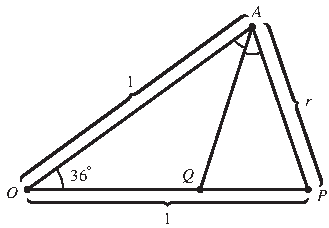
\includegraphics[width=0.452\linewidth,height=.8\textheight,keepaspectratio]{assets/p352_01.pdf}\end{center}
\begin{center}\small\textbf{41.13 Figure}\end{center}
\end{BookFloat}

\noindent In Exercises 6 through 9 use the results of Exercise 5 where needed to show that the statement is true.

\BookExercise{6.}{The regular 20-gon is constructible.}

\BookExercise{7.}{The regular 30-gon is constructible.}

\BookExercise{8.}{The angle \BookInline{72^{\circ }} can be trisected.}

\BookExercise{9.}{The regular 15-gon can be constructed.}

\BookExercise{10.}{Suppose you wanted to explain roughly in just three or four sentences, for a high school plane geometry teacher who never had a course in abstract algebra, how it can be shown that it is impossible to trisect an angle of \BookInline{60^{\circ }.} Write down what you would say.}

\BookExercise{11.}{Let \BookInline{S= \{n\in \mathbb{Z}\mid } an \BookInline{n} degree angle is constructible with a compass and straightedge\BookInline{\}.} We are assuming that if an angle of \BookInline{n} degrees is constructed, then \BookInline{n+ k(360)} is also constructed for any integer \BookInline{k.} Prove that \BookInline{S} is the principal ideal \BookInline{\langle 3\rangle \subseteq \mathbb{Z}.} It may be helpful to use Exercise 5.}

\BookExercise{12.}{The proof of Theorem 41.11 can be simplified by making a different choice of the angle \BookInline{\theta.} Find a constructible real number \BookInline{\alpha } so that the angle \BookInline{\theta = { \frac { \operatorname { a r c c o s } ( \alpha ) } { 3 } }} can be used in the formula cos \BookInline{3\theta = 4} cos\BookInline{3\theta - 3} cos \BookInline{\theta } to arrive at a polynomial that meets Eisenstein’s criteria. Then finish the proof of Theorem 4.11.}

\BookExercise{13.}{Prove that for at least one constructible angle \BookInline{5\theta,\allowbreak \theta } is not constructible.}

\BookExercise{14.}{Continuing Exercise 13,}

\BookExercise{a.}{Use Euler’s formula to show that for any integer \BookInline{n\geq 2,\allowbreak } cos\BookInline{(n\theta )= 2} cos\BookInline{(\theta )} cos\BookInline{((n- 1)\theta )- } cos\BookInline{((n- 2)\theta ).}}

\BookExercise{b.}{Use part a to rewrite cos\BookInline{(7\theta )} and use this formula to prove that there is a constructible angle \BookInline{7\theta } such that \BookInline{\theta } is not constructible.}

\BookExercise{c.}{For each integer \BookInline{1\leq n\leq 10,\allowbreak } is there a constructible angle \BookInline{n\theta } such that \BookInline{\theta } is not constructible?}

(The polynomials used in this exercise are called Chebyshev polynomials.)

\end{BookBody}
\ifdefined\BookMaster\let\BookFinish\relax\else\def\BookFinish{\end{document}}\fi\BookFinish
